\citeonline{apache:corte} explica que CGI é uma forma de interligação entre aplicativos externos com servidores de informação, do tipo servidores HTTP ou servidores web. Uma página HTML comum é composta por informações estáticas. Um programa CGI permite a montagem de uma página HTML em tempo real, com informações mais específicas ao interesse do usuário.

Por exemplo, digamos que se queira disponibilizar informações contidas em uma base de dados para qualquer usuário de um servidor de informações. Para isso, tem-se um formulário inicial, onde o usuário preenche determinadas informações e ao final, aciona um botão na tela, submetendo o pedido. Essas informações são passadas ao programa CGI, que processa essas informações, consulta uma base de dados e retorna as informações solicitadas através de uma página específica como pode ser visto na \autoref{fig:FEUP} \cite{apache:corte}.

Um programa CGI pode ser escrito em qualquer linguagem que permita ser executado no sistema. Contudo, esses programas necessitam residir em diretórios especiais (geralmente nomeado \textit{cgi-bin}), por questões de segurança e também para diferenciar de páginas comuns. Assim, o servidor sabe que esses programas devem ser executados e não simplesmente mostrados. Cada vez que o cliente pede o URL correspondente ao programa CGI, este é executado em tempo real, através da criação de um processo específico no servidor \cite{apache:corte}.

\begin{figure}[H]
    \centering
    \caption{Estrutura CGI}
    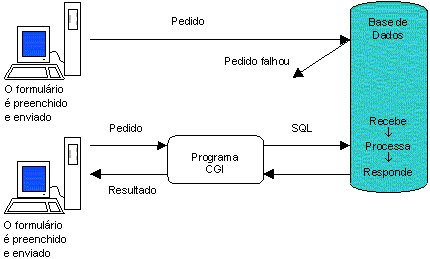
\includegraphics[width=0.7\textwidth]{./dados/figuras/fig11}
    \fonte{\citeonline{FEUP}}
    \label{fig:FEUP}
\end{figure}